\documentclass[11pt,a4paper]{article}
\usepackage{microtype}
\usepackage[margin=2.25cm,headheight=15pt]{geometry}
\usepackage{amsmath,amssymb,graphicx,booktabs,tabularx,array}
\usepackage[no-math]{fontspec}
\setmainfont{Times New Roman}
\setsansfont{Times New Roman}
\setmonofont{Times New Roman}
\usepackage[noOT1]{newtxmath}
\newcolumntype{Y}{>{\raggedright\arraybackslash}X}
\usepackage{xcolor,fancyhdr,titlesec,enumitem}
\makeatletter
\newcommand{\tableinput}[1]{\@@input #1 }
\makeatother
\usepackage[colorlinks=true,linkcolor=teal,citecolor=teal,urlcolor=teal]{hyperref}
\definecolor{teal}{HTML}{007F83}
\definecolor{ink}{HTML}{172F3E}
\definecolor{muted}{HTML}{536A78}
\definecolor{copper}{HTML}{CF703B}
\titleformat{\section}{\Large\sffamily\bfseries\color{ink}}{\color{teal}\thesection}{0.7em}{}
\titleformat{\subsection}{\large\sffamily\bfseries\color{ink}}{\thesubsection}{0.6em}{}
\pagestyle{fancy}\fancyhf{}
\fancyhead[L]{\small\sffamily\color{muted} NAVIER-STOKES IN TWO DIMENSIONS}
\fancyhead[R]{\small\sffamily\color{muted} LID-DRIVEN CAVITY}
\fancyfoot[L]{\small\sffamily\color{muted} Marouane Toumi}
\fancyfoot[R]{\small\sffamily\color{muted}\thepage}
\renewcommand{\headrulewidth}{0.3pt}
\setlength{\parindent}{0pt}\setlength{\parskip}{0.55em}
\setlist[itemize]{leftmargin=1.4em,itemsep=0.25em,topsep=0.2em}
\newcommand{\Rey}{\mathrm{Re}}
\newcommand{\dt}{\Delta t}
\newcommand{\code}[1]{\texttt{#1}}
\newcommand{\takeaway}[1]{\par\smallskip\noindent\colorbox{teal!7}{\parbox{\dimexpr\linewidth-2\fboxsep}{\textbf{\color{teal}Interpretation.} #1}}\par\smallskip}
\graphicspath{{../figures/}}
\hypersetup{pdftitle={Navier-Stokes in Two Dimensions: The Lid-Driven Cavity},pdfauthor={Marouane Toumi}}
\begin{document}
\hypersetup{pageanchor=false}
\begin{titlepage}
\vspace*{0.7cm}
{\sffamily\color{teal}\bfseries COMPUTATIONAL FLUID DYNAMICS \quad / \quad NUMERICAL STUDY\par}
\vspace{0.55cm}
{\sffamily\bfseries\color{ink}\fontsize{33}{38}\selectfont Navier-Stokes\\in two dimensions\par}
\vspace{0.45cm}
{\sffamily\Large\color{muted} The lid-driven cavity:\\approximation, verification, and what the flow reveals\par}
\vspace{0.55cm}
{\color{teal}\rule{\linewidth}{1.2pt}}
\vspace{0.25cm}
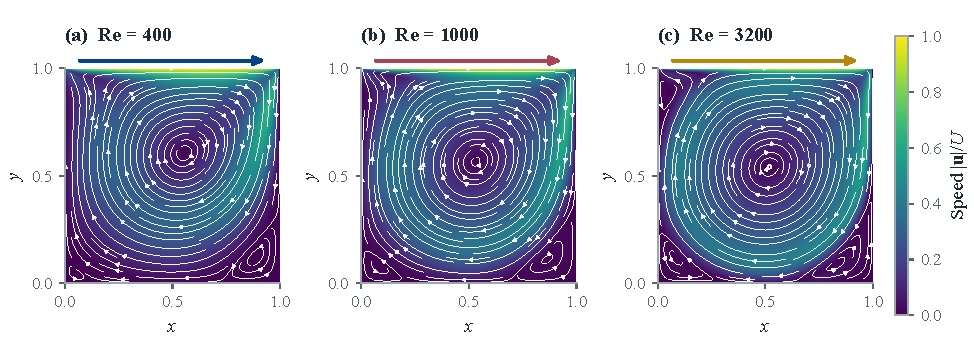
\includegraphics[width=\linewidth]{flow_atlas.pdf}\par
\vspace{0.3cm}
A moving lid generates a primary recirculation, thin wall layers, and secondary
corner vortices. This study follows those structures from the incompressible
Navier-Stokes equations to a working finite-difference implementation.
Each numerical choice is explained together with its cost, its verification,
and the limits of the resulting comparison with published data.

\begin{tabularx}{\linewidth}{@{}YYY@{}}
\textbf{Model} & \textbf{Method} & \textbf{Evidence}\\
2-D, viscous, incompressible & Vorticity-streamfunction & Manufactured solutions\\
Unit square, impulsive lid & Centered space, IMEX time & Two literature references
\end{tabularx}
\vfill
{\sffamily\large Marouane Toumi\par}
{\small\color{muted} Python package \code{ns2d} 1.3.0\quad |\quad Study revision: September 2026\par}
{\small\color{muted} Re = 400, 1000, 3200; three grids per case, fresh integrations, and measured accuracy budgets.}
\end{titlepage}
\hypersetup{pageanchor=true}

\section{Introduction}
Predicting the pressure drop in a pipe or the force of air on an aircraft wing
requires a mathematical description of how fluids move. The Navier-Stokes
equations provide that description for Newtonian fluids: they express
conservation of momentum, including the forces due to pressure and viscosity,
and are solved together with conservation of mass. In appropriate forms, and
coupled to additional physics, they also underpin models of atmospheric and
ocean circulation. Their importance comes from this ability to describe many
different flows using the same physical balances.

\subsection{From viscous forces to a mathematical model}
The equations emerged from nineteenth-century attempts to include internal
fluid friction in mechanics. In 1822, Claude-Louis Navier introduced viscous
forces into the equations of motion; George Gabriel Stokes developed his
formulation in 1845. Other researchers contributed to this development, so the
name records two major contributions to a longer history~\cite{bistafa}.
Viscosity accounts for the resistance between neighbouring fluid layers moving
at different velocities. It is essential for describing momentum transfer
from a solid wall to a fluid, which is precisely the mechanism studied here.

\subsection{Why solving the equations is difficult}
The main difficulty is the nonlinear transport term
$(\mathbf{u}\cdot\nabla)\mathbf{u}$: the velocity being sought also determines
how momentum is carried through the domain. A change in the flow therefore
changes its subsequent transport. In the incompressible formulation, pressure
must adjust throughout the domain to keep $\nabla\cdot\mathbf{u}=0$, coupling
the velocity components through a global constraint.

When inertia is strong relative to viscosity, thin wall layers and small
vortical structures can coexist with motion on the scale of the whole domain.
A numerical mesh must resolve the relevant spatial scales, while the time
step must satisfy both accuracy and stability requirements. Refining the mesh
increases the number of unknowns and can require more time steps. These costs,
together with complex boundaries, make general flows much harder to compute
than the special configurations for which exact solutions are available.

There is also a distinct mathematical question: for the three-dimensional
incompressible equations with smooth initial data, do smooth solutions always
persist, or can a singularity form? This is the subject of the Clay Millennium
problem~\cite{fefferman}. Global regularity is known for the corresponding
two-dimensional equations on the whole plane or with periodic boundary
conditions. The present cavity study
concerns numerical approximation in two dimensions; its discontinuous lid
velocity introduces boundary singularities of its own.

\subsection{How the lid-driven cavity became a benchmark}
The lid-driven cavity consists of a square with one moving wall and three
fixed walls. In 1966, Burggraf computed this flow up to
$\Rey=400$ and examined its primary circulation and secondary corner
eddies~\cite{burggraf1966}. Ghia, Ghia and Shin later published multigrid
solutions and velocity tables over a wider Reynolds-number range in
1982~\cite{ghia1982}; Botella and Peyret supplied a spectral reference at
$\Rey=1000$ in 1998~\cite{botella1998}. These studies provide independent
numerical comparisons for a geometry that still contains nonlinear transport,
wall layers and singular junctions between moving and stationary walls.

\clearpage
\subsection{The experiment and its objectives}
A square of side $L$ contains a Newtonian fluid of constant kinematic viscosity
$\nu$, initially at rest. At time zero the upper wall starts moving to the
right at speed $U$; the other three walls remain stationary. There is no imposed
pressure gradient. The moving wall supplies momentum, which spreads through
the fluid by advection and viscous diffusion.

This project follows the development of the circulation at
$\Rey=UL/\nu=400,1000,3200$. It asks how accurately the implementation
approximates the equations, how the computed fields change under grid and
time refinement, and how they compare with published cavity solutions.
Each question requires its own measurements: convergence of an iterative
solver alone cannot establish accuracy relative to the continuous equations.

\subsection{Scope and evidence}
The solver uses a uniform rectangular grid and a scalar streamfunction, so its
scope is two-dimensional, simply connected cavities with impermeable walls.
The production study uses the unit square and a unit lid. No turbulence model,
pressure reconstruction, variable viscosity, or three-dimensional instability
analysis is included.

The numerical comparisons use Ghia, Ghia and Shin~\cite{ghia1982} at three
Reynolds numbers, plus Botella and Peyret~\cite{botella1998} at $\Rey=1000$.
They are \emph{benchmark validation}: comparisons with independently computed
solutions of the same mathematical problem, not experimental validation of a
real apparatus.

\begin{tabularx}{\linewidth}{@{}>{\raggedright\arraybackslash}p{3.3cm}YY@{}}
\toprule
Question & Evidence supplied & Limit of the evidence\\\midrule
Implementation accuracy & Smooth manufactured solutions; space and time refinement & Does not establish the same global order at singular lid corners\\
Algebraic correctness & Poisson residual, divergence and circulation checks & Identities can hold on an inaccurate flow field\\
Benchmark agreement & Centerlines and primary vortex versus two papers & References have their own discretisation errors\\
Steady convergence & Update and steady-PDE residuals; ten-time-unit continuation & Measured drift is not a rigorous remaining-error bound\\
Discretisation sensitivity & Three grids per Re; transient time refinement & Richardson estimates assume a leading power-law error\\
\bottomrule
\end{tabularx}

\subsection{A guide to the report}
The report first derives the model, spatial stencils, wall treatment, and time
step. It then tests accuracy with a smooth manufactured solution, interprets
the cavity fields, and compares numerical references. The final section maps
the mathematics to the software and gives reproduction commands.

All nine production states were integrated from rest with the same numerical
kernel. Each record includes the case parameters, start and finish
timestamps, dependency versions, numerical-source fingerprint, runner
fingerprint, and hashes of the saved fields and cache, so that the results
builder can reject altered or unconverged production states. The manufactured
verification and cavity sensitivity experiments are separately reproducible.

\clearpage
\section{From velocity and pressure to two scalar fields}
\subsection{Nondimensional equations}
Scale lengths by $L$, velocities by $U$, time by $L/U$, pressure by $\rho U^2$,
vorticity by $U/L$, and streamfunction by $UL$. Dropping the dimensionless
asterisks gives
\begin{align}
\partial_t\mathbf{u}+(\mathbf{u}\cdot\nabla)\mathbf{u}
&=-\nabla p+\frac{1}{\Rey}\Delta\mathbf{u},\label{eq:ns}\\
\nabla\cdot\mathbf{u}&=0,\qquad \Rey=\frac{UL}{\nu},\qquad \mathbf{u}=(u,v).
\end{align}
Thus $\Rey$ measures the ratio of inertial to viscous effects. Time $t=1$ is
one lid travel time across the cavity.

Set
\begin{equation}
u=\psi_y,\qquad v=-\psi_x,\qquad
\omega=v_x-u_y=-\Delta\psi.\label{eq:definitions}
\end{equation}
The divergence vanishes because mixed derivatives commute. Taking the curl of
\eqref{eq:ns} eliminates pressure. In two dimensions the vortex-stretching term
vanishes, leaving
\begin{equation}
\boxed{\omega_t+\psi_y\omega_x-\psi_x\omega_y
=\Rey^{-1}\Delta\omega,\qquad -\Delta\psi=\omega.}\label{eq:transport}
\end{equation}
The convection sign follows directly from $u\omega_x+v\omega_y$ with
$u=\psi_y$, $v=-\psi_x$. The term is sometimes printed as
$\psi_x\omega_y-\psi_y\omega_x$; under the definitions \eqref{eq:definitions}
that expression equals $-\mathbf{u}\cdot\nabla\omega$ and has the wrong sign.
A positive lid speed drives a clockwise primary circulation: the primary
streamfunction is negative in this convention.

\subsection{Initial and boundary data}
On $\Omega=(0,1)^2$, the velocity is
\begin{equation}
(u,v)=\begin{cases}(1,0),&y=1,\quad 0<x<1,\\
(0,0),&\text{on the remaining open wall segments.}\end{cases}
\end{equation}
Impermeability makes $\psi$ constant along the connected boundary; choose that
constant as zero. Tangential no-slip supplies the normal derivative of $\psi$,
which will determine wall vorticity. The interior initial condition is rest:
$\psi=\omega=0$ at $t=0$.

The top corners are incompatible boundary junctions: the lid prescribes
$u=1$ while each side prescribes $u=0$. The impulsive start is also nonsmooth in
time. The solver does not smooth the lid, because that would define a different
benchmark. Stored corner velocities follow the side-wall convention; wall
vorticity at these singular points has no grid-independent point value.

\takeaway{The scalar formulation makes incompressibility straightforward and
removes pressure from the solve. The difficulty moves to the wall vorticity.
A velocity-pressure projection method would be more natural for extensions to
three dimensions; it is not required for this two-dimensional study.}

\clearpage
\section{Approximating space}
\subsection{Grid and finite differences}
Use $N_x\times N_y$ points, including the boundaries, with
$x_i=i h_x$, $y_j=j h_y$, $h_x=1/(N_x-1)$ and $h_y=1/(N_y-1)$.
Arrays use \code{field[i,j]}: $x$ is the first axis. A $129^2$ mesh has
$h=1/128$, not $1/129$.

For any smooth scalar field $q$, define
\begin{align}
D_xq_{ij}&=\frac{q_{i+1,j}-q_{i-1,j}}{2h_x},&
D_yq_{ij}&=\frac{q_{i,j+1}-q_{i,j-1}}{2h_y},\\
\Delta_hq_{ij}&=\frac{q_{i+1,j}-2q_{ij}+q_{i-1,j}}{h_x^2}
+\frac{q_{i,j+1}-2q_{ij}+q_{i,j-1}}{h_y^2}.\label{eq:lap}
\end{align}
Taylor expansion yields, for example,
$D_xq=q_x+(h_x^2/6)q_{xxx}+O(h_x^4)$. The interior spatial truncation error is
second order when the required derivatives remain bounded.

The transport term is evaluated in advective form:
\begin{equation}
C_h(\psi,\omega)_{ij}=(D_y\psi)_{ij}(D_x\omega)_{ij}
-(D_x\psi)_{ij}(D_y\omega)_{ij}.\label{eq:conv}
\end{equation}
It uses the current streamfunction and vorticity, including the wall values
needed by the first interior row of centered differences.

\subsection{Why use these approximations?}
\begin{tabularx}{\linewidth}{@{}>{\raggedright\arraybackslash}p{3.1cm}YY@{}}
\toprule
Choice & Benefit & Cost or alternative\\\midrule
Uniform grid & Transparent stencils; separable Poisson operator & Many nodes are spent in the smooth core rather than thin wall layers\\
Centered convection & Second-order consistency without a first-order upwind diffusion term & No general monotonicity guarantee; under-resolved oscillations are possible\\
Five-point Laplacian & Compact SPD Dirichlet system & Second-order spatial accuracy; smoothness assumptions fail at lid corners\\
Advective Jacobian & Direct implementation of $u\omega_x+v\omega_y$ & Does not inherit the energy/enstrophy properties of an Arakawa Jacobian\\
\bottomrule
\end{tabularx}

Arakawa's construction~\cite{arakawa1966} is an important alternative when
preserving the quadratic invariants of inviscid two-dimensional advection is
a priority. This implementation uses the simpler centered product and makes
no claim of exact energy or enstrophy conservation. In the viscous driven
cavity, the moving boundary supplies energy and diffusion dissipates it, so
the energy itself should not be constant during the transient.

\takeaway{Formal order describes the local approximation of smooth fields.
Resolution and boundary regularity determine whether that order is visible in
a particular cavity observable.}

\clearpage
\section{How the moving wall creates vorticity}
The Poisson equation needs one boundary value for $\psi$. With $\psi=0$
already imposed, the no-slip information is transferred to $\omega$.
At the top wall, away from the corners, Taylor expansion gives
\begin{equation}
\psi(x,1-h_y)=-h_y u_T+\frac{h_y^2}{2}\psi_{yy}(x,1)+O(h_y^3).
\end{equation}
Because $\psi$ is constant along that wall, $\psi_{xx}=0$ there. Hence
$\psi_{yy}=-\omega$ and
\begin{equation}
\boxed{\omega_{i,N_y-1}=-\frac{2\psi_{i,N_y-2}}{h_y^2}
-\frac{2u_T(x_i)}{h_y}.}\label{eq:thom}
\end{equation}
This is the Thom wall formula. A lid moving to the right produces negative
vorticity next to an initially motionless interior, as expected for clockwise
rotation.

For general tangential wall velocities, the other formulas are
\begin{align}
\omega_{i,0}&=-2\psi_{i,1}/h_y^2+2u_B(x_i)/h_y,\\
\omega_{0,j}&=-2\psi_{1,j}/h_x^2-2v_L(y_j)/h_x,\\
\omega_{N_x-1,j}&=-2\psi_{N_x-2,j}/h_x^2+2v_R(y_j)/h_x.
\end{align}
In the standard cavity, $u_T=1$ and the other velocities vanish.

\subsection{Local order is not global order}
Dividing the Taylor remainder by $h^2$ leaves an $O(h)$ wall truncation error.
That does not by itself establish a first-order global streamfunction error:
the wall error enters a coupled elliptic and transport problem. The observed
global order must be measured. Section~\ref{sec:verification} finds approximately second-order
streamfunction and vorticity convergence with the Thom wall treatment on the
selected smooth manufactured field, over a horizon long enough for
wall-generated errors to reach the interior. This
is consistent with the role of local vorticity formulas discussed by
E and Liu~\cite{eliu1996}; it is not a universal guarantee for a singular cavity.

\subsection{What the corner convention means}
No interior five-point Laplacian or centered convection stencil reaches a
corner. Changing the four stored corner vorticities therefore leaves the
computed interior unchanged. This implementation stores the sum of the two
adjacent wall formulas at each corner. That convention makes a particular
trapezoidal circulation identity exact; it is bookkeeping for integration,
not a physical evaluation of the singularity.

The displayed wall vorticity is lagged by one step: it was constructed from
$\psi^n$, whereas the stored interior is $\omega^{n+1}$. This distinction
matters when checking circulation or interpreting transient wall values.

\takeaway{The wall formula is the mechanism that drives this solver. A
verification field with zero tangential wall velocities cannot test its
velocity-dependent terms.}

\clearpage
\section{Advancing time and solving the systems}
\subsection{One semi-implicit step}
Let $L=-\Delta_h$ on the interior with homogeneous Dirichlet conditions.
Let $b^n$ contain the Thom wall ring from $\psi^n$, with zero interior.
The algorithm performs
\begin{align}
(I+\dt\Rey^{-1}L)\omega_I^{n+1}
&=\omega_I^n-\dt C_h(\psi^n,\omega^n)
+\dt\Rey^{-1}(\Delta_h b^n)_I+\dt f_I^{n+1},\label{eq:step}\\
L\psi_I^{n+1}&=\omega_I^{n+1},\qquad \psi^{n+1}|_{\partial\Omega}=0.
\end{align}
The source $f$ vanishes for the cavity and is used only for manufactured
solutions. In exact-wall verification, the diffusion solve instead uses the
known wall vorticity at $t^{n+1}$. Convection always uses the current-time wall
values. Explicit convection, backward Euler diffusion, and the lagged wall
treatment make this a \emph{first-order} time scheme.

The wall-ring term in \eqref{eq:step} is simply Dirichlet-column elimination.
For example, the node below the lid receives
$+(\dt/\Rey h_y^2)\omega_{i,N_y-1}^{n}$ on its right-hand side.
No nonlinear iteration is performed.

\subsection{Why the linear solves are well behaved}
The Dirichlet negative Laplacian is symmetric positive definite. Therefore
both $L$ and $I+\dt\Rey^{-1}L$ are suitable for conjugate gradient.
On this uniform rectangle, a faster default is available: the type-I discrete
sine transform diagonalises $L$. Its eigenvalues are
\begin{equation}
\lambda_{pq}=\frac{4}{h_x^2}\sin^2\!\frac{p\pi}{2(N_x-1)}
+\frac{4}{h_y^2}\sin^2\!\frac{q\pi}{2(N_y-1)}.
\end{equation}
For $(\alpha I+\beta L)z=r$, transform $r$, divide each coefficient by
$\alpha+\beta\lambda_{pq}$, and inverse transform. The solve is exact up to
floating-point error for the \emph{discrete} system, at
$O(M\log M)$ cost for $M=(N_x-2)(N_y-2)$ unknowns.

Two alternative backends serve as checks: sparse LU, factored once and reused,
and conjugate gradient with an incomplete-Cholesky IC(0) preconditioner.
The latter is SPD; a generic incomplete-LU preconditioner would not provide
that required property. Iterative solutions agree to the requested tolerance,
not necessarily bit for bit.

\subsection{When is a run steady?}
The driver monitors the interior update rate
\begin{equation}
R_n=\frac{\|\omega_I^{n+1}-\omega_I^n\|_\infty}{\dt}.
\end{equation}
The production stopping threshold is $10^{-6}$, tested every 50 steps.
It is an absolute update-rate criterion, not an estimate of spatial error.
A fixed-step run stops at the first time at or beyond its requested $T$;
the final step is not shortened and can overshoot by less than $\dt$.
The production time caps are safeguards, not declarations that a flow has
settled. Every reported production state must meet the criterion. The accuracy
study then checks a further ten time units with both $\dt$ and $\dt/2$.

\clearpage
\section{Stability: the interior and the walls}
Implicit diffusion removes the usual explicit interior diffusion restriction,
but it does not make the full algorithm unconditionally stable.
For constant advection velocity $(a,b)$ on an infinite uniform grid, a Fourier
mode has amplification factor
\begin{equation}
G=\frac{1-i\dt A}{1+\nu\dt B},\quad
A=\frac{a\sin\theta_x}{h_x}+\frac{b\sin\theta_y}{h_y},\quad
B=\frac{4\sin^2(\theta_x/2)}{h_x^2}
+\frac{4\sin^2(\theta_y/2)}{h_y^2},
\end{equation}
where here $\nu=1/\Rey$. Since $A^2\leq(a^2+b^2)B$, a sufficient bound for
this \emph{linear interior} analysis is
\begin{equation}
\dt\leq\frac{2\nu}{a^2+b^2}.
\end{equation}
This argument assumes constant coefficients and does not include the cavity
walls or nonlinear interactions.

\subsection{A boundary experiment on the implemented step}
Turn convection off, set all wall velocities to zero, and reconstruct $\psi$
from each interior basis vector of $\omega$. One step gives a linear map
$\omega_I^{n+1}=M\omega_I^n$. The module \code{ns2d.stability} builds $M$ using
the production step and computes its spectral radius. With
$d=\nu\dt/h^2$, the measured crossings of $\rho(M)=1$ are
\begin{center}
\begin{tabular}{@{}lrrr@{}}\toprule
Grid & $17^2$ & $25^2$ & $33^2$\\\midrule
Critical $d$ & 1.58085 & 1.54647 & 1.53199\\\bottomrule
\end{tabular}
\end{center}
The finite-grid trend motivates using $d_{\max}=1.5$ with a safety factor.
Prescribing a fixed zero wall-vorticity ring removes this feedback mechanism.
These tests diagnose a boundary restriction; they do not prove a sharp
nonlinear threshold or a theorem for stretched rectangular grids.

The default helper combines the three safeguards
\begin{equation}
\dt=s\min\!\left(\frac{h_{\min}}{U_*},\frac{2}{\Rey U_*^2},
1.5\Rey h_{\min}^2\right),\qquad s=0.5,
\end{equation}
where $U_*$ is an estimated maximum speed. The cavity constructor uses the
configured lid-speed magnitude. A new flow configuration should be checked
with a smaller step; the helper is not an adaptive stability controller.

\subsection{A mesh diagnostic is not a stability theorem}
The cell Reynolds number is $\Rey_h=\Rey Uh$ (unit lid: $\Rey_h=\Rey h$).
The familiar $\Rey_h\leq2$ condition concerns monotonicity of a one-dimensional
steady centered advection-diffusion stencil. It is a useful warning about
resolution, not a universal cavity accuracy or temporal-stability criterion.
On the $257^2$ grids here it is 1.56, 3.91, and 12.5. Reducing $\dt$ cannot
substitute for resolving a thin wall layer.

\clearpage
\section{Verification with a known smooth solution}\label{sec:verification}
Choose the manufactured streamfunction
\begin{equation}
\psi_e=\sin(\pi x)\sin(\pi y)e^{-t}
+\tfrac12\sin(2\pi x)\sin(2\pi y)e^{-2t},\qquad
\omega_e=-\Delta\psi_e.
\end{equation}
It vanishes on the boundary but has nonzero normal derivatives there, so the
wall velocities exercise the moving-wall terms. Its two Laplacian eigenvalues
differ; consequently $\omega_e$ is not proportional to $\psi_e$ and convection
does not vanish identically.

Symbolic differentiation defines the continuous forcing
\begin{equation}
f=\partial_t\omega_e+(\partial_y\psi_e)(\partial_x\omega_e)
-(\partial_x\psi_e)(\partial_y\omega_e)-\Rey^{-1}\Delta\omega_e.
\end{equation}
This is a continuous manufactured source, not a discrete source chosen to make
the numerical answer exact. All tests use $\Rey=100$ and start from the exact
continuous fields; the initial pair need not satisfy the discrete Poisson
relation exactly.

\subsection{Errors and observed order}
Use the composite trapezoidal norm
\begin{equation}
\|e\|_{2,h}=\left(h_xh_y\sum_{ij}\sigma_{ij}e_{ij}^2\right)^{1/2},
\qquad p=\frac{\log(E_h/E_{h/2})}{\log2},
\end{equation}
where $\sigma$ is 1 inside, $1/2$ on an edge, and $1/4$ at a corner.
The four inert vorticity corners are excluded from both vorticity norms without
renormalising other weights; the streamfunction norms use the full grid.

\begin{itemize}
\item \textbf{Space:} $N=17,33,65,129$, fixed $\dt=5\times10^{-6}$, $T=0.5$.
Run both exact wall vorticity and the production Thom wall treatment.
\item \textbf{Time:} fixed $65^2$ grid, $T=0.032$, with
$\dt=3.2,1.6,0.8,0.4\times10^{-4}$. Compare to a same-grid solution with
$\dt_{\mathrm{ref}}=2.5\times10^{-6}$ to reduce the spatial-error floor.
\item \textbf{Joint refinement:} $N=17,33,65$, $T=0.5$ and
$\dt=4\times10^{-4}(h/h_{17})^2$.
\end{itemize}
The spatial horizon matters. The diffusion length $\sqrt{T/\Rey}\approx0.07$
spans about one cell on the $17^2$ grid and nine cells on the $129^2$ grid, so
vorticity errors generated at the walls reach the interior. Over a much
shorter horizon such as $T=0.005$, about 96-99\% of the streamfunction error
would be the Poisson discretisation error of the exact initial vorticity, and
the test would exercise neither the transport step nor the wall treatment.

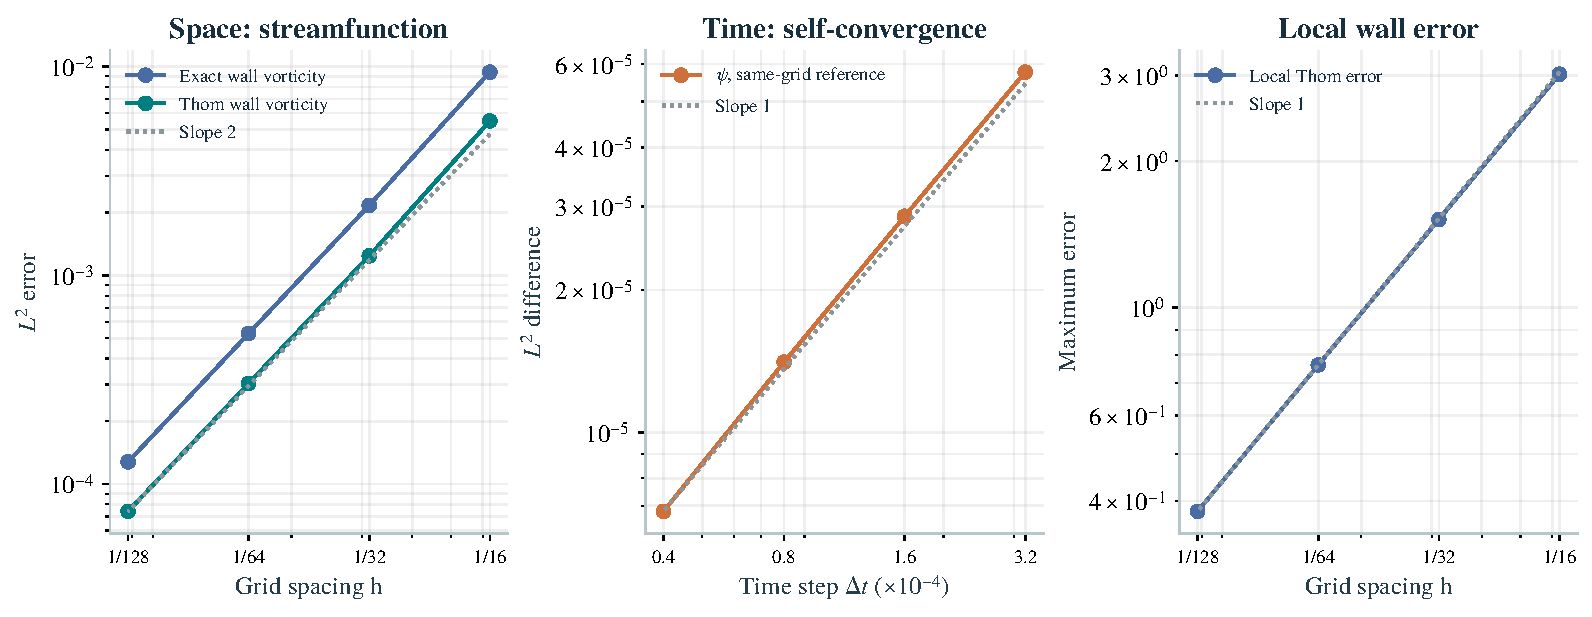
\includegraphics[width=\linewidth]{verification.pdf}\par
{\small\color{muted}(a) Spatial streamfunction error ($L^2$), (b) temporal
self-convergence ($L^2$ difference from the same-grid reference), and (c) local
wall truncation error (maximum over the four walls). Dotted guides show the
expected slopes; legend values $p$ are the observed orders on the finest pair.}

\clearpage
\subsection{What the convergence measurements say}
\begin{tabularx}{\linewidth}{@{}Xl@{}}\toprule
Measurement & Successive observed orders\\\midrule
Spatial $\psi$, exact wall $\omega$, $L^2$ & 2.119, 2.040, 2.043\\
Spatial $\omega$, exact wall $\omega$, $L^2$ & 2.110, 2.038, 2.042\\
Spatial $\psi$, Thom wall $\omega$, $L^2$ & 2.147, 2.029, 2.036\\
Spatial $\omega$, Thom wall, $L^2$ & 2.144, 2.040, 2.044\\
Spatial $\omega$, Thom wall, maximum norm & 1.858, 1.995, 2.029\\
Temporal $\psi$, same-grid reference, $L^2$ & 1.011, 1.023, 1.047\\
Joint refinement $\psi$, $L^2$ & 2.154, 2.025\\\bottomrule
\end{tabularx}

The measurements support second-order spatial accuracy for this smooth test,
with Thom as well as exact wall vorticity, and first-order time accuracy.
The exact-wall vorticity row tests the discrete transport equation directly,
since that run receives exact wall values. Only the Thom maximum-norm
vorticity order on the coarsest pair (1.86) departs noticeably from 2; the
local $O(h)$ wall error is largest there. The Thom errors are smaller because
the wall error partly cancels the interior error, so error levels do not rank
the wall treatments. For an ideal first-order error, differences from the
finite temporal reference scale like $\dt-\dt_{\mathrm{ref}}$; this bias alone
predicts the measured orders 1.011, 1.023 and 1.047.

Two additional checks challenge the setup. An asymmetric field,
\[
\psi_e=\sin(\pi x)\sin(2\pi y)e^{-t}+0.3\sin(3\pi x)\sin(\pi y)e^{-2t},
\]
integrated to $T=0.5$ on
$17^2,33^2,65^2$ grids, gives streamfunction orders 2.29 and 2.00 (the $17^2$
grid is pre-asymptotic). On the $129^2$ grid, doubling $\dt$ to $10^{-5}$
changes the streamfunction $L^2$ error by about 3\%, so the temporal
contribution shifts the observed orders by at most about 0.04. These checks
make it unlikely that symmetry or temporal contamination produced the
spatial slope. All errors are in the JSON evidence.

\subsection{Algebraic checks and their interpretation}
For reconstructed velocity, the centered mixed differences cancel:
\begin{equation}
D_xu+D_yv=D_xD_y\psi-D_yD_x\psi=0.
\end{equation}
The cancellation also holds next to impermeable straight walls with the
implemented boundary velocities. The Poisson residual measures a different
identity:
\begin{equation}
r_P=\|\Delta_h\psi+\omega_I\|_\infty.
\end{equation}
Both quantities are recomputed for every cavity state and exported in
\code{data/validation.json}; the Poisson audit requires $r_P<10^{-8}$.

For a vorticity field constructed consistently from one $\psi$, the wall
formulas, interior Laplacian and sum corner convention telescope under the
trapezoidal rule:
\begin{equation}
h_xh_y\sum_{ij}\sigma_{ij}\omega_{ij}
=\oint_{\partial\Omega}\mathbf{u}\cdot d\boldsymbol\ell=-1.
\end{equation}
Here the contour orientation is counterclockwise. The implementation of
\code{circulation\_identity} constructs its own interior $-\Delta_h\psi$;
it checks the discrete formulas and quadrature, not the independently stored
Poisson solution. The latter is checked by $r_P$. Direct integration of stored
$\omega$ also includes its one-step wall lag.

Tests additionally compare DST, LU and CG, check invariance to inert corner
values, and compare a checkpoint restart with uninterrupted stepping. These
checks constrain different failure modes. None replaces the refinement study.

\takeaway{The verification evidence is strong for the selected smooth problem.
It should not be reinterpreted as proof of second-order accuracy for every
quantity in the singular lid-driven cavity.}

\clearpage
\section{What the cavity flow reveals}
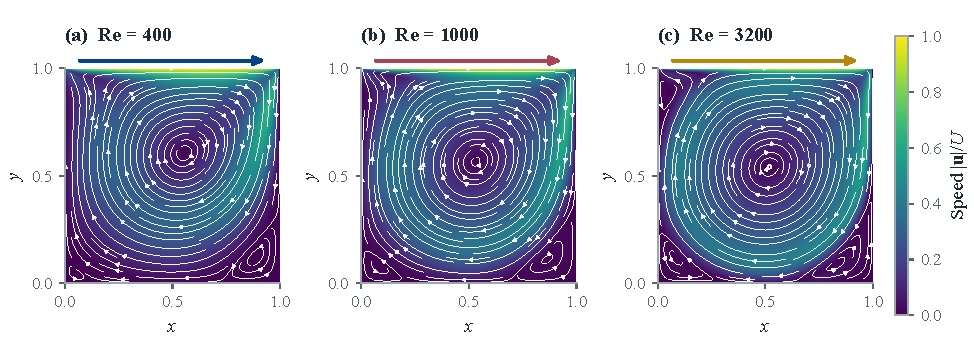
\includegraphics[width=0.92\linewidth]{flow_atlas.pdf}\par
{\small\color{muted}Velocity streamlines over speed on $257^2$ grids. The common
colour scale is 0-1 in lid-speed units. These are instantaneous streamlines,
not particle trajectories through the transient.}

The lid first creates a shear layer. Fluid moves right beneath it, turns down
the right wall, returns along the bottom, and rises along the left wall. The
primary circulation is clockwise. As $\Rey$ increases, viscous transport
becomes weaker relative to advection, wall gradients sharpen, and the primary
vortex moves toward the cavity centre. Counter-rotating corner cells become
more prominent; at $\Rey=3200$ a top-left cell is visible.

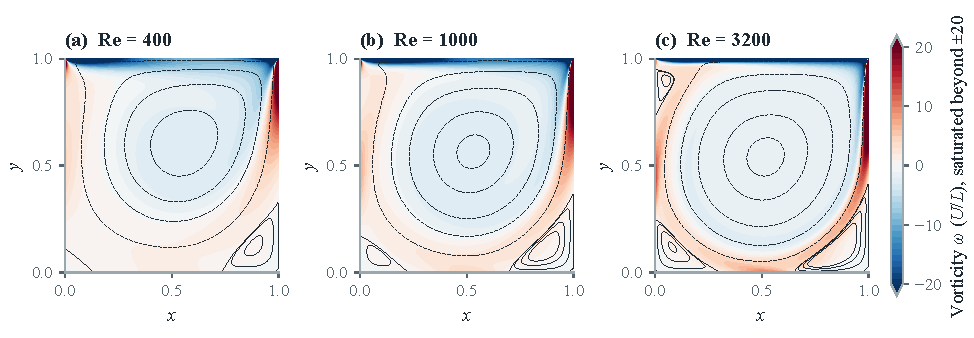
\includegraphics[width=0.92\linewidth]{vorticity.pdf}\par
{\small\color{muted}Vorticity with streamfunction contours; negative (clockwise) levels are
dashed. The same range
$[-20,20]$ is used in all panels. Saturated colours hide larger magnitudes;
the full fields, including the lid-corner values, are not clipped in the data.}

The vorticity field exposes the wall layers more clearly than a streamline
plot. Fine structure near walls is also where centered advection on a coarse
mesh is most vulnerable. A smooth-looking streamline plot alone is therefore
an inadequate accuracy check.

\clearpage
\subsection{Secondary circulation at the corners}
The primary vortex carries most of the visible motion, but it is not the only
recirculation in the cavity. Near a corner the main flow can turn away from
both walls and leave a small region rotating in the opposite direction.
In the present sign convention those counter-rotating cells have positive
streamfunction. They occupy a much smaller range of $\psi$ than the primary
vortex, so a uniform set of contour levels over the whole cavity can miss them.

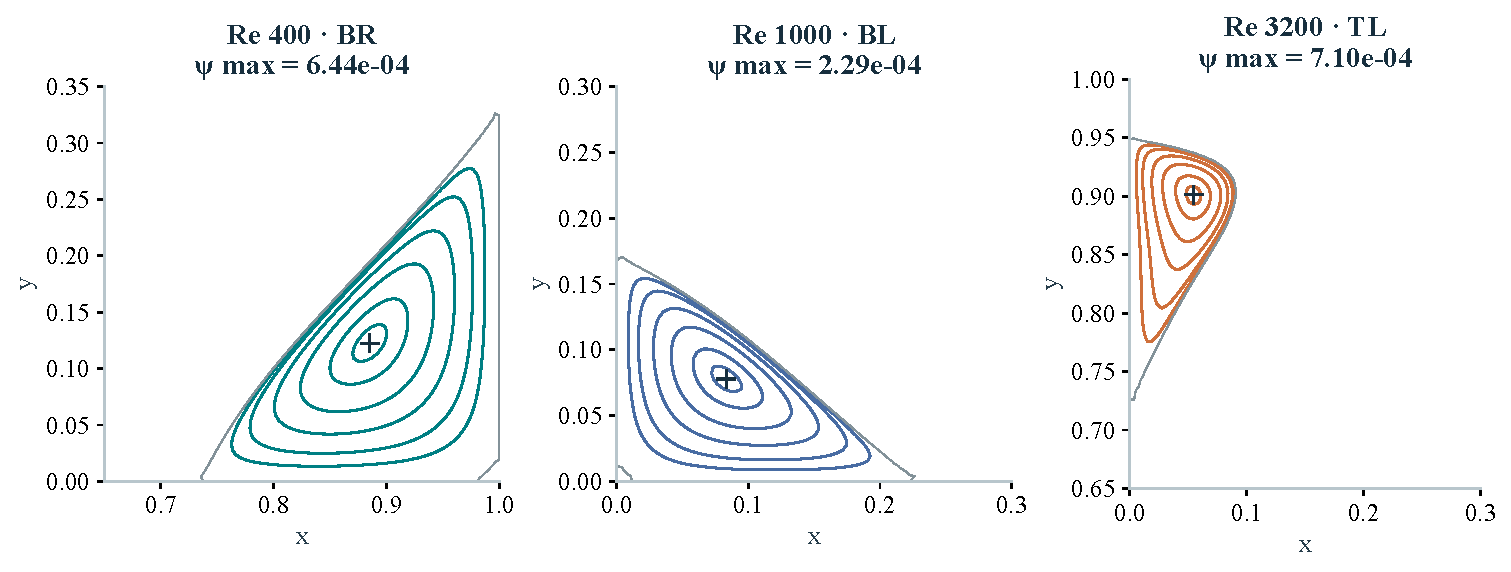
\includegraphics[width=0.92\linewidth]{corner_eddies.pdf}\par
{\small\color{muted}Selected positive-streamfunction corner cells. Contour
levels are fractions of each local maximum, so colours do not compare vortex
strength across panels. Crosses mark local quadratic-fit extrema.}


\begin{center}
\begin{tabular}{@{}llrrr@{}}\toprule
Case & Selected cell & $\psi_{\max}$ & $x$ & $y$\\\midrule
\tableinput{eddy_rows.tex}
\bottomrule
\end{tabular}
\end{center}
{\small\color{muted}Selected extrema of the present $257^2$ fields, found by
local quadratic fits. They are computed quantities, not reference values.
Scientific notation ``e'' denotes powers of ten. Grid sensitivity of the
bottom-right cell is included in the accuracy study.}

Each zoom uses levels at 5, 15, 35, 60, 85 and 97 percent of that cell's
maximum. This reveals its shape while making the normalisation explicit.
A cross marks the fitted extremum; the zero contour separates positive
streamfunction from the clockwise primary circulation. Contour appearance
must therefore not be used to compare strengths without the numbers above.

These eddies are a useful resolution test. Their amplitudes are orders of
magnitude smaller than the primary streamfunction, and their wall gradients
are sampled by relatively few nodes on a uniform mesh. Good agreement in
primary-vortex strength does not imply equal accuracy for every small cell.
The current search finds the strongest positive cell in each corner quadrant;
it is not an exhaustive detector of nested higher-order vortices.

\takeaway{A figure can reveal flow structure only at the scales it displays.
Global plots explain the circulation; local plots and explicit contour levels
make the smaller features interpretable.}

\clearpage
\section{Convergence and comparison with Ghia}
The reported primary vortex is a local quadratic fit around the grid minimum
of $\psi$. It reduces node-location quantisation but is not a new high-order
flow solution. The relative discrepancy in its strength is
$100|\psi_{\min}-\psi_{\mathrm{ref}}|/|\psi_{\mathrm{ref}}|$.

\begin{center}\small
\begin{tabular}{@{}rrrrcrr@{}}\toprule
$\Rey$ & Grid & Final $t$ & $R$ & Steady? & $\psi_{\min}$ & Difference (\%)\\\midrule
\tableinput{results_rows.tex}
\bottomrule\end{tabular}
\end{center}
{\small\color{muted}Reference strengths: $-0.113909$, $-0.117929$, and
$-0.120377$ for Re = 400, 1000, 3200 respectively (Ghia, Table V).
Scientific notation ``e'' denotes a power of ten.}

All nine integrations meet the same $10^{-6}$ stopping threshold. The final
times differ because settling depends on both Reynolds number and grid.
The following accuracy study reports the change during a further ten time
units and explicitly compares earlier $t=150$ or $t=300$ snapshots with the
converged fine-grid states. A residual threshold alone is not an error bound.

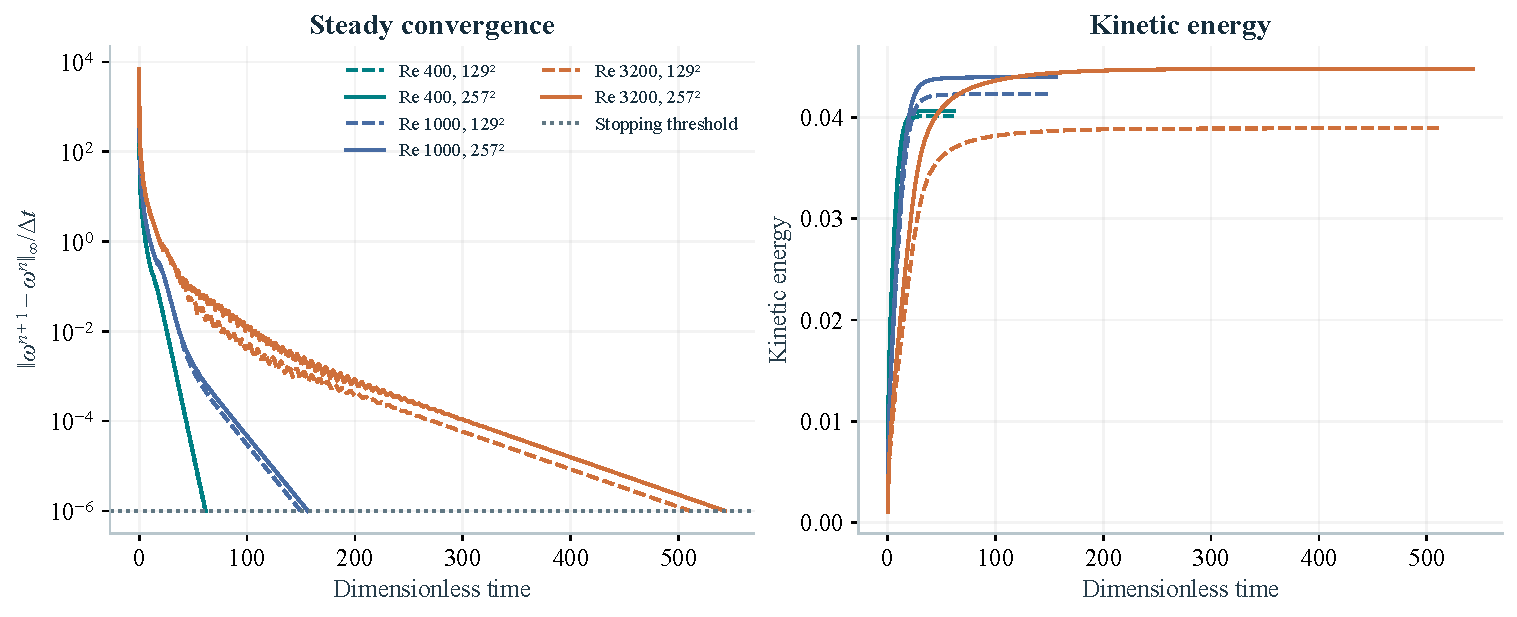
\includegraphics[width=\linewidth]{residuals.pdf}\par
{\small\color{muted}Recorded (a) interior update residuals and (b) kinetic energy on
the $129^2$ (dashed, open markers) and $257^2$ (solid, filled markers) grids.
Colour and marker shape both identify the Reynolds number.
The threshold is $10^{-6}$. Energy is a global diagnostic and can appear almost
constant while the maximum update residual remains above the threshold.}

\subsection{What grid refinement supports}
The primary-vortex comparison improves with refinement. Other observables
need individual checks: at $\Rey=400$, for example, the unflagged RMS
discrepancy of $v$ on the horizontal centerline does not decrease between
$129^2$ and $257^2$.
The next section measures differences between our own grids, independently of
Ghia's values, and reports conditional Richardson estimates rather than
equating benchmark agreement with continuum accuracy.

\clearpage
\subsection{Centerline profiles, with every reference point visible}
\begin{center}
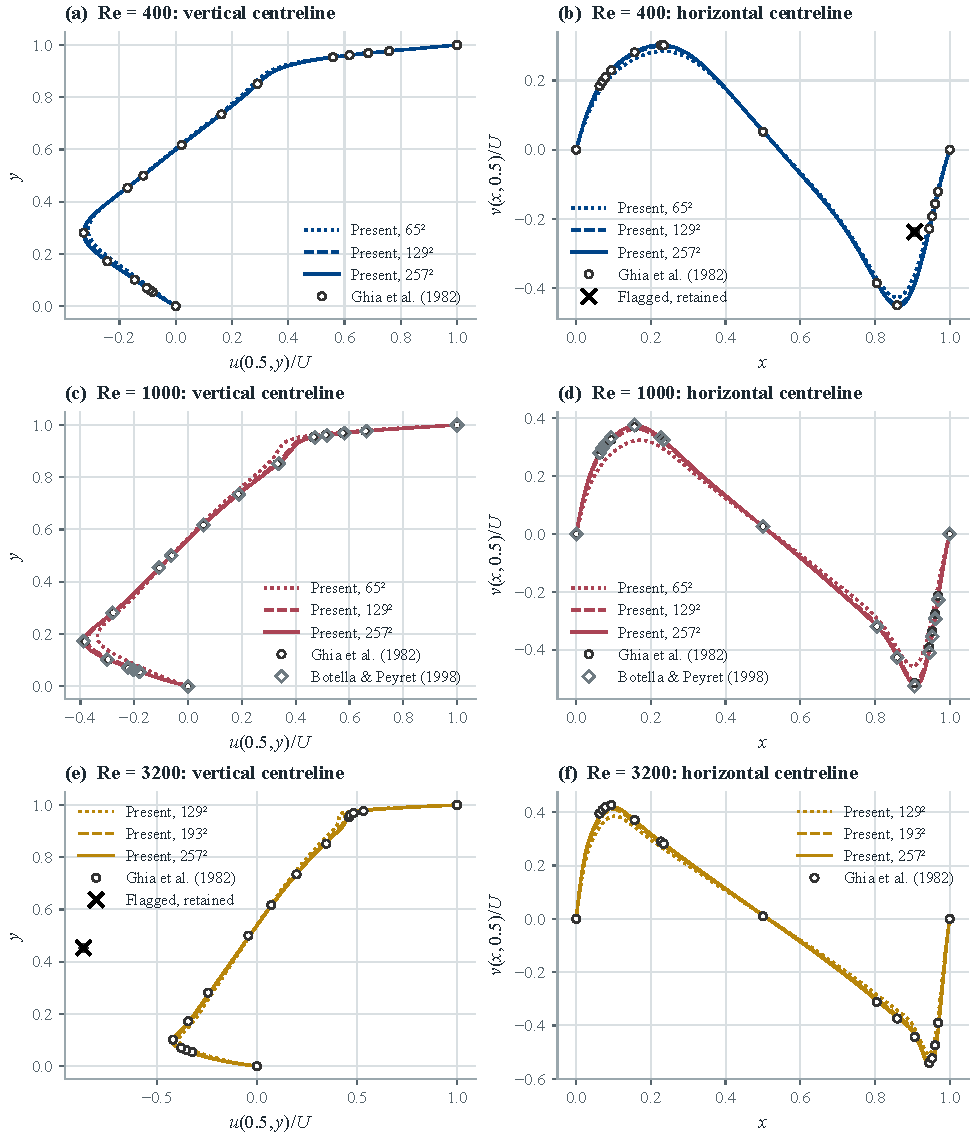
\includegraphics[width=0.91\linewidth]{centerlines.pdf}\par
\end{center}
{\small\color{muted}Computed profiles are drawn from the full grid;
line style distinguishes the grids (dotted, dashed, solid from coarse to
fine). Open circles are the published Ghia stations; black crosses flag
suspect published values but retain them in the headline RMS. Open grey
diamonds at Re = 1000 show the reflected Botella-Peyret reference. The Re = 1000 and 3200 curves are
states that meet the common steady criterion. Their remaining drift is
measured in the accuracy study.}

\clearpage
\subsection{Reference anomalies and reproducible metrics}
For $m=17$ reference stations, the profile error is
\begin{equation}
E_{u,\mathrm{RMS}}=\sqrt{\frac{1}{m}\sum_{k=1}^{m}
\left[u_h(0.5,y_k)-u_{\mathrm{ref},k}\right]^2},
\end{equation}
and likewise for $v$. Linear interpolation evaluates the numerical fields
at the printed coordinates. The wall stations, where the velocity is
prescribed ($u=0$ at $y=0$, $u=1$ at $y=1$, $v=0$ at $x=0,1$), are included;
they contribute zero error and therefore lower the RMS. This is an absolute
dimensionless velocity error, not a percentage.

The original paper was inspected at Tables I and II (pp.\ 398-399) and
Table V (pp.\ 408-409). Two anomalous stations affect this study:
\begin{itemize}
\item At $\Rey=3200$, Table I prints $u=-0.86636$ at $y=0.4531$.
It is retained. Replacing it by $-0.086636$ based on the current computation
would use the answer under test to alter the reference.
\item At $\Rey=400$, Table II prints $v=-0.23827$ at $x=0.9063$.
It is retained; a second RMS shows the effect of excluding that one point.
\end{itemize}
These are flags for interpretation, not claims of an official erratum.

\begin{center}\small
\begin{tabular}{@{}rrrrrr@{}}\toprule
$\Rey$ & Grid & $u$ all & $u$ unflagged & $v$ all & $v$ unflagged\\\midrule
\tableinput{profile_rows.tex}
\bottomrule\end{tabular}
\end{center}
{\small\color{muted}Full and secondary RMS errors. ``Unflagged'' uses 16
stations in the affected component and 17 otherwise. All station values,
interpolated results and flags are exported in
\code{data/centerline\_comparisons.csv}.}

The primary-vortex reference is not one uniform $129^2$ data set. Table V
explicitly lists $257^2$ at $\Rey=400$ and $129^2$ at $\Rey=1000,3200$.
The printed $\Rey=3200$ centre $x=0.5165$ is retained even though it is off
the listed mesh. We do not infer or repair a reference by rounding it to a
preferred grid.

\takeaway{Raw reference data and a transparent sensitivity calculation make
an anomalous comparison inspectable. A smaller score obtained after changing
the source values would be much harder to interpret.}

\clearpage
\section{An independent spectral reference at Re = 1000}
Botella and Peyret~\cite{botella1998} use Chebyshev collocation and subtract
leading corner singularities. This provides a useful second numerical method
against which to compare the finite-difference result. Their Tables 6, 9 and
10 supply the primary vortex and both centerlines.

\subsection{Reconciling the lid direction}
Their lid moves left. Reflect the field about $x=1/2$ to compare with the
right-moving lid used here:
\begin{align}
x_R&=1-x_L,\qquad y_R=y_L,\\
u_R(x_R,y)&=-u_L(1-x_R,y),&v_R(x_R,y)&=v_L(1-x_R,y),\\
\psi_R(x_R,y)&=-\psi_L(1-x_R,y).
\end{align}
In particular, $v$ does \emph{not} change sign. After reflection, the reference
primary vortex is $\psi=-0.1189366$ at $(0.5308,0.5652)$.
The code preserves the left-lid tabulation and applies the transformation
explicitly when constructing the comparison.

\begin{center}
\begin{tabular}{@{}lrrr@{}}\toprule
Quantity & Present, $257^2$ & Ghia & Botella-Peyret\\\midrule
\tableinput{botella_rows.tex}
\bottomrule
\end{tabular}
\end{center}

\subsection{What this changes in the interpretation}
Agreement with Ghia is close, but it is not a continuum error bar. The
primary-vortex strength and the $u$ profile on the vertical centerline are
closer to Ghia, whereas the $v$ profile on the horizontal centerline and the
vortex ordinate are closer to the spectral reference. The comparison reveals the
size and direction of differences between reference methods. It also shows
why one small percentage cannot summarise every feature of the flow.

The present field meets the common steady threshold, and
Section~\ref{sec:accuracy} measures its remaining drift. The spectral reference reports
higher accuracy in its own convergence study, but benchmark discrepancies
still combine errors of both methods. Our three-grid study supplies a distinct,
explicitly conditional estimate of our discretisation uncertainty.

\takeaway{A useful numerical portfolio explains why an answer should be
trusted, how it compares with more than one method, and where the evidence
stops. These discrepancies are part of the result.}

\clearpage
\section{Separating grid, time and settling effects}\label{sec:accuracy}
All measurements in this section are generated by \code{scripts/run\_accuracy.py}
and retained in \code{data/accuracy.json}. They use the same cavity equations,
wall treatment and interior stencils as the production study.

\subsection{A three-grid estimate independent of the benchmarks}
For $\Rey=400,1000$ use $N=65,129,257$. For $\Rey=3200$ use
$N=129,193,257$, avoiding the very coarse $65^2$ grid in the order estimate.
Each state starts from rest and reaches the same steady threshold. Write
$h_c>h_m>h_f$ for the coarse, medium and fine spacings. For a scalar observable
$q$, assume a leading error model
\begin{equation}
q(h)=q_0+C h^p,\qquad
\frac{q_c-q_m}{q_m-q_f}
=\frac{h_c^p-h_m^p}{h_m^p-h_f^p}.\label{eq:richardson}
\end{equation}
The latter equation is solved for $p$ using the actual spacings; no equal-ratio
formula is imposed on the $\Rey=3200$ sequence. It gives
\begin{equation}
q_0^{\rm est}=q_f+\frac{q_f-q_m}{(h_m/h_f)^p-1},\qquad
U_h=1.25\frac{|q_f-q_m|}{(h_m/h_f)^p-1}.
\end{equation}
The corresponding relative grid-convergence index is $100U_h/|q_f|$,
following the three-grid safety factor of Celik et al.~\cite{celik2008}.
Non-monotone sequences, roundoff-level differences, and sequences with no
positive fitted order in $(0.01,10)$ receive no extrapolation.

\begin{center}\small
\begin{tabular}{@{}rlrrr@{}}\toprule
$\Rey$ & $N$ values & Fitted $p$ & $\psi_{\min,0}^{\rm est}$ & GCI (\%)\\\midrule
\tableinput{grid_rows.tex}
\bottomrule\end{tabular}
\end{center}
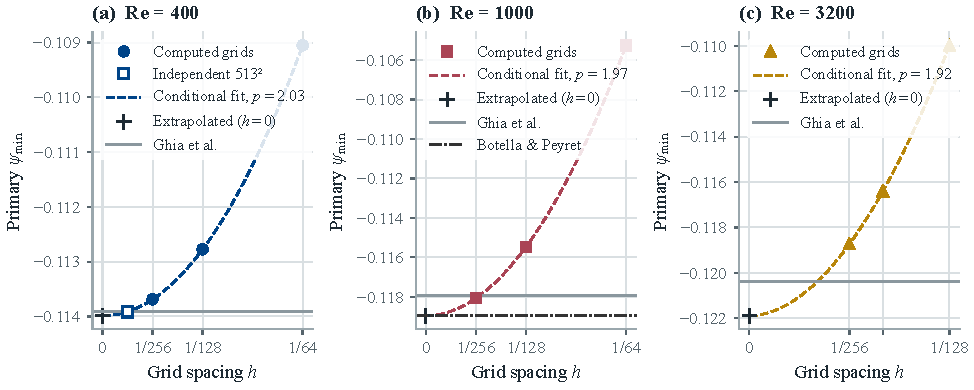
\includegraphics[width=\linewidth]{grid_convergence.pdf}
{\small\color{muted}Computed primary streamfunctions and conditional fits.
The point at $h=0$ is an extrapolation, not an additional simulation.
Reference lines do not enter the fit.}

Three data points determine the three model parameters; a successful fit is
therefore not an independent test of the power-law assumption. These are
engineering uncertainty estimates, not guaranteed bounds or statistical
confidence intervals. The fitted $p$ belongs to this observable and grid range,
not to every quantity produced by the solver.

\clearpage
\subsection{An independent fourth-grid check at Re = 400}
An additional $513^2$ run starts from rest and meets the same stopping
criterion. Comparing overlapping triples tests the original extrapolation:
\begin{center}\small
\begin{tabular}{@{}lrrr@{}}\toprule
$N$ values & Fitted $p$ & Extrapolated $\psi_{\min}$ & Fine-grid GCI (\%)\\\midrule
\tableinput{fourth_grid_rows.tex}
\bottomrule\end{tabular}
\end{center}
The original three-grid model predicts $\psi_{\min}=-0.1139135$ on $513^2$; the independent integration gives $-0.1139144$, a difference of $9.51\times10^{-7}$. The two extrapolated limits differ by $1.67\times10^{-6}$. This is an independent check of the primary-streamfunction model at $\Rey=400$ only. It does not establish the same reliability for other Reynolds numbers or observables.


\subsection{Other observables and complete centerline differences}
The same procedure is applied to the vortex coordinates, kinetic energy,
center vorticity, and bottom-right secondary-vortex strength.

\begin{center}\footnotesize
\begin{tabular}{@{}rlrrl@{}}\toprule
$\Rey$ & Observable & Fitted $p$ & GCI (\%) & Interpretation\\\midrule
\tableinput{observable_rows.tex}
\bottomrule\end{tabular}
\end{center}

Profile differences use 65 common, uniformly spaced grid nodes, including
the endpoints; no interpolation is needed. Their $L^2$ norm uses composite
trapezoidal integration on $[0,1]$, distinct from the RMS over Ghia's
17 irregularly spaced stations.

\begin{center}\small
\begin{tabular}{@{}rlrr@{}}\toprule
$\Rey$ & Grid pair & $\|\delta u\|_{2}$ & $\|\delta v\|_{2}$\\\midrule
\tableinput{grid_profile_rows.tex}
\bottomrule\end{tabular}
\end{center}

At $\Rey=400$, the bottom-right eddy strength is non-monotone across the
three grids, so no GCI is assigned. At $\Rey=3200$, the kinetic-energy GCI
is $6.695\%$, versus $3.321\%$ for the primary streamfunction. Position
estimates also depend on the local quadratic fit used to locate the extremum.

\takeaway{The main vortex's uncertainty estimate cannot be transferred to
secondary eddies or to the whole velocity field.}

\clearpage
\subsection{Time refinement at a common transient time}
For each Reynolds number, integrate afresh from rest on the same $129^2$ grid
to $T=5$ with $\dt$, $\dt/2$, and $\dt/4$. The target is an integer multiple
of every step. Define
\begin{equation}
D_u(\dt)=\|u_{\dt}(1/2,\cdot,T)-u_{\dt/2}(1/2,\cdot,T)\|_2,
\quad p_{t,u}=\log_2\frac{D_u(\dt)}{D_u(\dt/2)},
\end{equation}
and similarly for $v$. Using a common grid isolates temporal self-convergence
from spatial refinement. It does not measure the continuum error at that grid.

\begin{center}\small
\begin{tabular}{@{}rrrrrr@{}}\toprule
$\Rey$ & Base $\dt$ & $D_u(\dt)$ & $D_u(\dt/2)$ & $p_{t,u}$ & $p_{t,v}$\\\midrule
\tableinput{time_rows.tex}
\bottomrule\end{tabular}
\end{center}
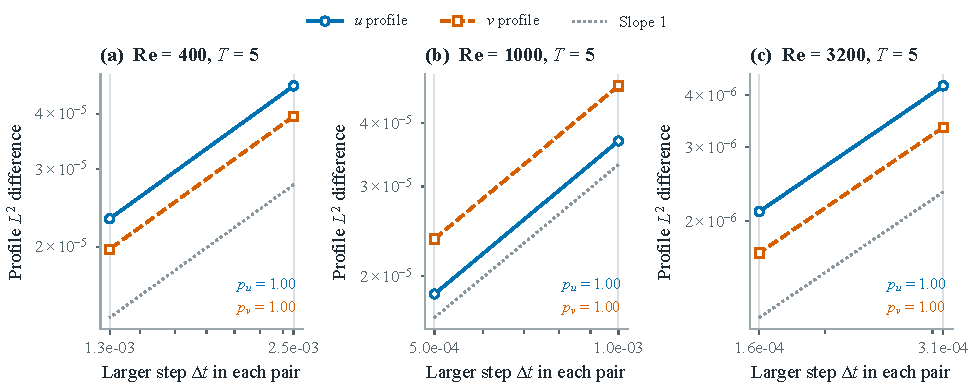
\includegraphics[width=\linewidth]{cavity_time_convergence.pdf}
{\small\color{muted}Successive profile differences from actual cavity
transients. All runs use the impulsively started, discontinuous unit lid.}

\subsection{Why a steady solution has a different time-step question}
At an exactly stationary discrete state, $\omega^{n+1}=\omega^n=\omega$
and the lagged boundary is also stationary. Subtracting $\omega$ from
\eqref{eq:step} and dividing by $\dt$ gives
\begin{equation}
C_h(\psi,\omega)-\Rey^{-1}\Delta_h\omega=0.
\end{equation}
Thus the time step cancels out of the fixed-point equations. There is no
separate backward-Euler truncation bias in their exactly converged solution.
The step still affects transient accuracy, stability, and how closely the
iteration approaches that fixed point. Different stable steps can also have
different attraction behavior if multiple discrete solutions exist.

This is why the time-order experiment is performed during the transient.
For the final states, halving the step is instead used as a continuation
sensitivity check, together with an unfiltered steady-equation residual.

\clearpage
\subsection{Measure settling instead of relying only on a threshold}
Refresh the wall vorticity from the current $\psi$ and evaluate
\begin{equation}
F_h=C_h(\psi,\omega)-\Rey^{-1}\Delta_h\omega,\qquad
R_{\rm PDE}=\|F_h\|_\infty.
\end{equation}
The monitored update rate is related to the old-state defect by
$(I+\dt\Rey^{-1}L)(\omega^{n+1}-\omega^n)/\dt=-F_h$.
It is therefore a filtered residual, not numerically identical to $R_{\rm PDE}$.

Starting independently from each saved final state, integrate ten further
time units with the original step and with half that step. The following
table reports the initial steady defect, the largest monitored update rate
across both continuations, and the larger observable drift of the two trials.
Halving the step reduces the implicit filtering, so its initial update rate
can marginally exceed the original stopping threshold even though the initial
fields are identical. These small excursions are retained; the original-step
stopping criterion is not retroactively changed.

\begin{center}\small
\begin{tabular}{@{}rrrrrrr@{}}\toprule
$\Rey$ & Grid & $R_{\rm PDE}$ & $R_{\max}$ & $|\delta\psi_{\min}|$ & $\|\delta u\|_2$ & $\|\delta v\|_2$\\\midrule
\tableinput{settling_rows.tex}
\bottomrule\end{tabular}
\end{center}

This measures sensitivity over a specified interval. It is not a proof that
all later changes are smaller, and the residual is not divided by an
unjustified decay constant to manufacture an error bound.

The fresh fine-grid integrations also save intermediate states. Comparing
the former observation times to the converged states quantifies the effect
that was previously left unresolved:
\begin{center}\small
\begin{tabular}{@{}rrrrr@{}}\toprule
$\Rey$ & Earlier $t$ & $\psi_{\min}$ change (\%) & $\|\delta u\|_2$ & $\|\delta v\|_2$\\\midrule
\tableinput{transient_rows.tex}
\bottomrule\end{tabular}
\end{center}

\begin{center}\small
\begin{tabular}{@{}rrrr@{}}\toprule
$\Rey$ & Grid GCI (\%) & Settling drift (\%) & Step-halving $|\delta\psi_{\min}|$\\\midrule
400 & 0.327 & 1.830e-05 & 5.49e-13\\
1000 & 0.941 & 7.603e-05 & 5.48e-13\\
3200 & 3.321 & 7.843e-05 & 5.01e-13\\
\bottomrule\end{tabular}\end{center}
The three columns are distinct sensitivity measures on the $257^2$ grids, not independent random errors to combine in quadrature. The first assumes a power-law spatial error; the second measures ten-time-unit drift; the last compares the endpoints of the two continuations. The measured settling effects can thus be assessed against spatial sensitivity without treating the residual threshold as an uncertainty estimate.
Across these three fine-grid cases, the conditional grid estimate is at least $1.24\times10^{4}$ times the measured primary-vortex settling drift. Within these experiments, spatial resolution is the dominant measured limitation for primary-vortex strength. This conclusion does not transfer automatically to every flow quantity.


\takeaway{The completed experiments distinguish measured settling, transient
time accuracy, conditional grid uncertainty, and disagreement with a numerical
reference. Each answers a different question about the computed flow.}


\clearpage
\section{Software design and reproduction}
\begin{tabularx}{\linewidth}{@{}p{3.5cm}Y@{}}\toprule
Module & Responsibility\\\midrule
\code{grid.py} & Coordinates, array layout, spacing and validated dimensions\\
\code{operators.py} & Stencils, sparse matrices, DST/LU/CG, step-size guidance\\
\code{boundary.py} & Four Thom wall formulas and corner storage convention\\
\code{problems.py} & Cavity data, symbolic manufactured forcing, restart signature\\
\code{solver.py} & One time step, monitoring, snapshots and checked restart\\
\code{postproc.py} & Velocity, extrema, quadrature and algebraic diagnostics\\
\code{benchmark.py} & Published data, explicit flags, coordinate transformation\\
\code{verification.py} & Spatial, temporal and joint refinement experiments\\
\code{accuracy.py} & Observable differences, steady defect and conditional grid extrapolation\\
\bottomrule\end{tabularx}

Checkpoints include the mesh lengths, time step, boundary configuration, and
built-in problem parameters. Strict loading rejects incompatible states before
changing the solver. An explicit non-strict import is available for continuing
an old state under a deliberately changed configuration. Custom problems must
include all physical parameters in their checkpoint signature. Restart with
DST and the same configuration is tested bit for bit; changing backends only
promises agreement within solver tolerance.

\subsection{Reproduce the project from its root directory}
\begin{verbatim}
python -m pip install -e ".[dev,notebook]"
python -m pytest -q
python scripts/run_demo.py
python scripts/run_production.py --force
python scripts/check_fourth_grid.py
python scripts/run_accuracy.py
python scripts/build_results.py
python scripts/build_notebook.py --execute
python scripts/build_report.py
\end{verbatim}
The demonstration uses a small $65^2$ grid. The production suite is much more
expensive, especially $\Rey=3200$. Field caches are deliberately excluded from
Git; committed figures, tables, measured JSON evidence and the executed
notebook remain readable without them. The report build requires Tectonic or
a TeX Live installation. See \code{docs/reproducibility.md} for partial builds
and the precise provenance of saved results.

\subsection{Next numerical experiments}
The next useful accuracy experiment extends the fourth-grid check from
$\Rey=400$ to the higher Reynolds numbers and to wall-sensitive observables.
An Arakawa advection option and higher-order time integration with a compatible
wall update are separate method extensions. Grid stretching could target boundary layers but would require
replacing the present sine-transform diagonalisation. A smoothed lid is useful
for a separate regularity study and should be labelled as a different problem.

The current result is a compact, inspectable demonstration of solving,
verifying and interpreting the two-dimensional Navier-Stokes equations.
Its strongest claims are the ones connected directly to reproducible tests
and published comparison data.

\clearpage
\begin{thebibliography}{9}
\bibitem{bistafa}
S.~R.~Bistafa. 200 Years of the Navier-Stokes Equation.
\href{https://arxiv.org/abs/2401.13669}{arXiv:2401.13669}.

\bibitem{fefferman}
C.~L.~Fefferman. Existence and smoothness of the Navier-Stokes equation.
Official Millennium Prize problem description, Clay Mathematics Institute.
\href{https://www.claymath.org/wp-content/uploads/2022/06/navierstokes.pdf}{Problem statement}.

\bibitem{burggraf1966}
O.~R.~Burggraf (1966).
Analytical and numerical studies of the structure of steady separated flows.
\emph{Journal of Fluid Mechanics}, 24(1), 113-151.
\href{https://doi.org/10.1017/S0022112066000545}{doi:10.1017/S0022112066000545}.

\bibitem{ghia1982}
U.~Ghia, K.~N.~Ghia and C.~T.~Shin (1982).
High-Re solutions for incompressible flow using the Navier-Stokes equations
and a multigrid method.
\emph{Journal of Computational Physics}, 48(3), 387-411.
\href{https://doi.org/10.1016/0021-9991(82)90058-4}{doi:10.1016/0021-9991(82)90058-4}.

\bibitem{botella1998}
O.~Botella and R.~Peyret (1998).
Benchmark spectral results on the lid-driven cavity flow.
\emph{Computers \& Fluids}, 27(4), 421-433.
\href{https://doi.org/10.1016/S0045-7930(98)00002-4}{doi:10.1016/S0045-7930(98)00002-4}.

\bibitem{eliu1996}
W.~E and J.-G.~Liu (1996).
Vorticity boundary condition and related issues for finite difference schemes.
\emph{Journal of Computational Physics}, 124(2), 368-382.
\href{https://doi.org/10.1006/jcph.1996.0066}{doi:10.1006/jcph.1996.0066}.

\bibitem{arakawa1966}
A.~Arakawa (1966).
Computational design for long-term numerical integration of the equations of
fluid motion: two-dimensional incompressible flow. Part I.
\emph{Journal of Computational Physics}, 1(1), 119-143.
\href{https://doi.org/10.1016/0021-9991(66)90015-5}{doi:10.1016/0021-9991(66)90015-5}.

\bibitem{celik2008}
I.~B.~Celik, U.~Ghia, P.~J.~Roache, C.~J.~Freitas, H.~Coleman and P.~E.~Raad (2008).
Procedure for estimation and reporting of uncertainty due to discretization in CFD applications.
\emph{Journal of Fluids Engineering}, 130(7), 078001.
\href{https://doi.org/10.1115/1.2960953}{doi:10.1115/1.2960953}.
\end{thebibliography}

\vspace{1cm}
\textbf{Data provenance.} The comparison arrays were checked against the
original tables. The paper scans are not redistributed in this repository.
Source links, flags, and the Botella-Peyret reflection are documented in
\code{docs/references.md}. The simulation and verification measurements are
exported as machine-readable files under \code{data/}.

\textbf{Reading the figures.} All flow figures are generated from numerical
fields. Streamlines show the instantaneous velocity direction. Vorticity colour
limits and local eddy contour normalisations are explicitly stated. No generated
illustration is used as evidence of a computed solution.
\end{document}
